\documentclass[tikz,border=2pt]{standalone}
\usepackage{amsmath,amssymb}
\usepackage{tikz}
\usetikzlibrary{arrows.meta}

\begin{document}
% Two sets have the same cardinality when their elements can be paired off by a bijection;
% this works for finite sets by counting and for infinite sets without counting at all.
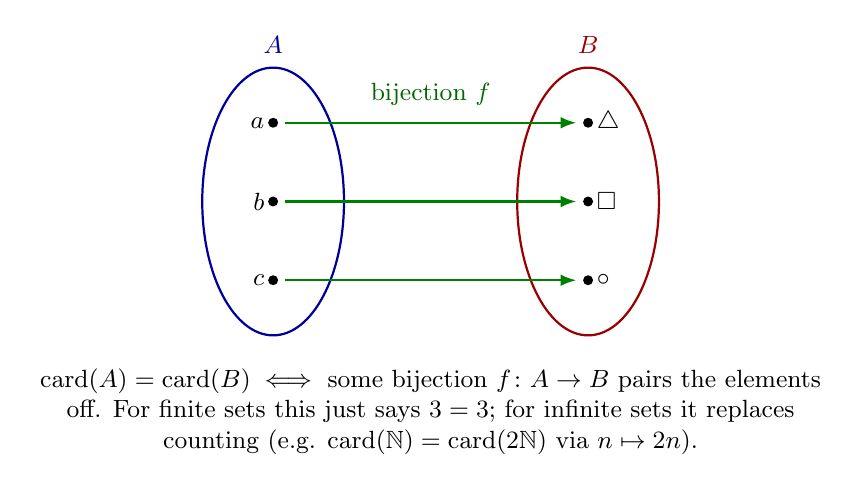
\begin{tikzpicture}[every node/.style={font=\small}, >={Latex[length=2mm]}]
	\draw[thick, blue!60!black] (0,0) ellipse (0.9 and 1.7);
	\draw[thick, red!60!black] (4,0) ellipse (0.9 and 1.7);
	\node[blue!60!black, anchor=south] at (0,1.75) {$A$};
	\node[red!60!black, anchor=south] at (4,1.75) {$B$};
	\foreach \y/\a/\b in {1/a/\triangle, 0/b/\square, -1/c/\circ} {
		\fill (0,\y) circle (1.8pt) node[left, inner sep=3pt] {$\a$};
		\fill (4,\y) circle (1.8pt) node[right, inner sep=3pt] {$\b$};
		\draw[->, green!50!black, thick] (0.15,\y) -- (3.85,\y);
	}
	\node[green!40!black, anchor=south] at (2,1.1) {bijection $f$};
	\node[anchor=north, align=flush center, text width=10cm] at (2,-2.0) {$\operatorname{card}(A)=\operatorname{card}(B)\iff$ some bijection $f\colon A\to B$ pairs the elements off. For finite sets this just says $3=3$; for infinite sets it replaces counting (e.g. $\operatorname{card}(\mathbb{N})=\operatorname{card}(2\mathbb{N})$ via $n\mapsto2n$).};
\end{tikzpicture}
\end{document}
